% Chapter 3, Section 3: Expectation, Variance, and Covariance

\section{Expectation, Variance, and Covariance}
\label{sec:expectation-variance}

\subsection{Intuition: Characterizing Random Variables}

When we have a random variable, we often want to summarize its behavior with a few key numbers:
\begin{itemize}
    \item \textbf{Expected value (mean)}: The "center" or "typical" value
    \item \textbf{Variance}: How much the values spread out from the center
    \item \textbf{Covariance}: How two variables move together
\end{itemize}

Think of it like describing a person:
\begin{itemize}
    \item \textbf{Mean height}: The average height of people in a group
    \item \textbf{Variance in height}: How much heights vary (tall vs short people)
    \item \textbf{Covariance of height and weight}: Do taller people tend to weigh more?
\end{itemize}

\subsection{Expectation}

The \textbf{expected value} or \textbf{mean} of a function $f(x)$ with respect to distribution $P(x)$ is:

For discrete variables:
\begin{equation}
\mathbb{E}_{x \sim P}[f(x)] = \sum_{x} P(x) f(x)
\end{equation}

For continuous variables:
\begin{equation}
\mathbb{E}_{x \sim p}[f(x)] = \int p(x) f(x) \, dx
\end{equation}

\subsubsection{Example: Expected Value of Dice}

For a fair six-sided die:
\begin{align}
\mathbb{E}[X] &= \sum_{x=1}^{6} x \cdot P(X=x) \\
&= 1 \cdot \frac{1}{6} + 2 \cdot \frac{1}{6} + \cdots + 6 \cdot \frac{1}{6} \\
&= \frac{1+2+3+4+5+6}{6} = \frac{21}{6} = 3.5
\end{align}

The expected value is 3.5, even though we can never actually roll 3.5!

\begin{figure}[h]
\centering
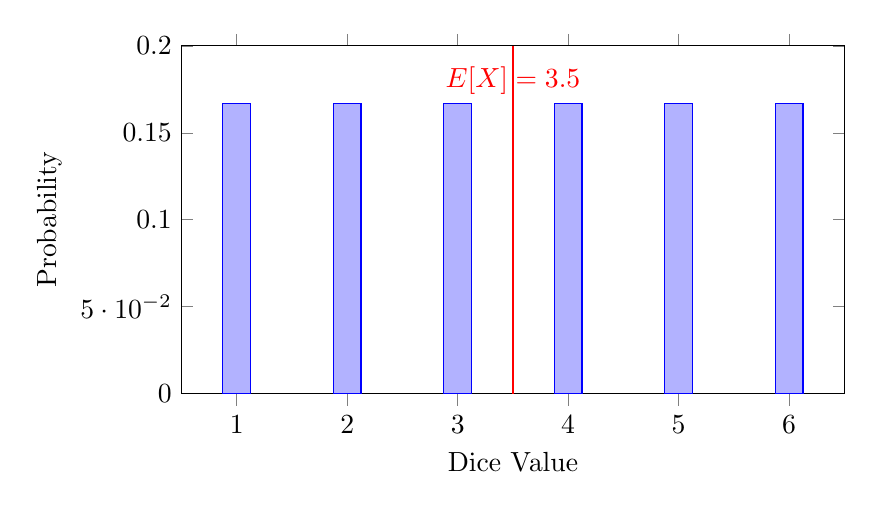
\begin{tikzpicture}
\begin{axis}[
    ybar,
    ylabel={Probability},
    xlabel={Dice Value},
    xtick={1,2,3,4,5,6},
    ymin=0,
    ymax=0.2,
    width=10cm,
    height=6cm
]
\addplot coordinates {(1,1/6) (2,1/6) (3,1/6) (4,1/6) (5,1/6) (6,1/6)};
\draw[red, thick] (axis cs:3.5,0) -- (axis cs:3.5,0.2);
\node[red] at (axis cs:3.5,0.18) {$\mathbb{E}[X] = 3.5$};
\end{axis}
\end{tikzpicture}
\caption{Probability distribution of a fair die with expected value marked}
\label{fig:dice-expectation}
\end{figure}

\subsection{Variance}

\subsubsection{Intuition: Measuring Spread}

Variance tells us how "spread out" the values are around the mean. Think of two dart players:
\begin{itemize}
    \item \textbf{Low variance}: All darts cluster tightly around the bullseye
    \item \textbf{High variance}: Darts are scattered all over the board
\end{itemize}

The \textbf{variance} measures the spread of a distribution:

\begin{equation}
\text{Var}(X) = \mathbb{E}[(X - \mathbb{E}[X])^2] = \mathbb{E}[X^2] - (\mathbb{E}[X])^2
\end{equation}

The \textbf{standard deviation} is $\sigma = \sqrt{\text{Var}(X)}$.

\subsubsection{Example: Variance of Dice}

For our fair die:
\begin{align}
\text{Var}(X) &= \mathbb{E}[X^2] - (\mathbb{E}[X])^2 \\
&= \left(\frac{1^2 + 2^2 + \cdots + 6^2}{6}\right) - (3.5)^2 \\
&= \frac{91}{6} - 12.25 = 15.17 - 12.25 = 2.92
\end{align}

So $\sigma = \sqrt{2.92} \approx 1.71$.

\begin{figure}[h]
\centering
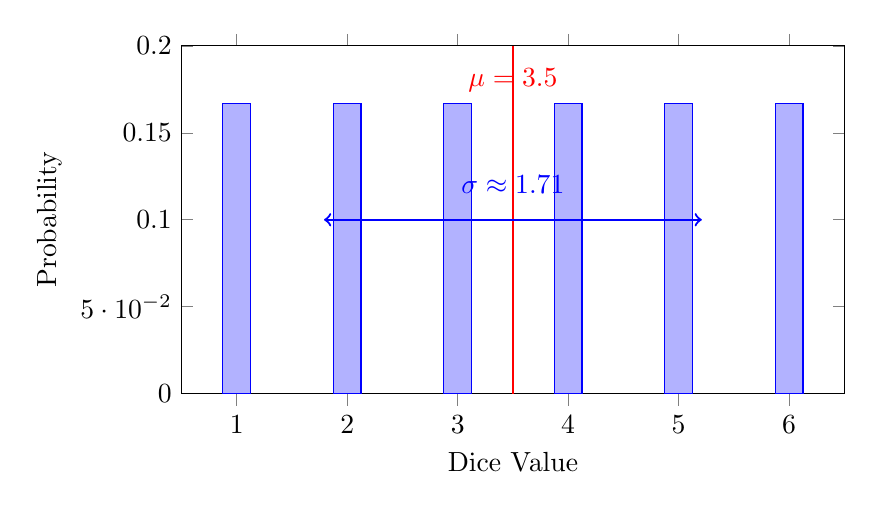
\begin{tikzpicture}
\begin{axis}[
    ybar,
    ylabel={Probability},
    xlabel={Dice Value},
    xtick={1,2,3,4,5,6},
    ymin=0,
    ymax=0.2,
    width=10cm,
    height=6cm
]
\addplot coordinates {(1,1/6) (2,1/6) (3,1/6) (4,1/6) (5,1/6) (6,1/6)};
\draw[red, thick] (axis cs:3.5,0) -- (axis cs:3.5,0.2);
\node[red] at (axis cs:3.5,0.18) {$\mu = 3.5$};
\draw[blue, thick, <->] (axis cs:1.79,0.1) -- (axis cs:5.21,0.1);
\node[blue] at (axis cs:3.5,0.12) {$\sigma \approx 1.71$};
\end{axis}
\end{tikzpicture}
\caption{Probability distribution showing mean and standard deviation}
\label{fig:dice-variance}
\end{figure}

\subsection{Covariance}

\subsubsection{Intuition: How Variables Move Together}

Covariance tells us whether two variables tend to move in the same direction or opposite directions:
\begin{itemize}
    \item \textbf{Positive covariance}: When one goes up, the other tends to go up too
    \item \textbf{Negative covariance}: When one goes up, the other tends to go down
    \item \textbf{Zero covariance}: No clear relationship
\end{itemize}

Examples:
\begin{itemize}
    \item \textbf{Height and weight}: Positive covariance (taller people tend to weigh more)
    \item \textbf{Price and demand}: Negative covariance (higher prices usually mean lower demand)
    \item \textbf{Height and IQ}: Near zero covariance (no clear relationship)
\end{itemize}

The \textbf{covariance} measures how two variables vary together:

\begin{equation}
\text{Cov}(X, Y) = \mathbb{E}[(X - \mathbb{E}[X])(Y - \mathbb{E}[Y])]
\end{equation}

Positive covariance indicates that $X$ and $Y$ tend to increase together, while negative covariance indicates they tend to vary in opposite directions.

\subsubsection{Example: Height and Weight}

Consider a small dataset of people:
\begin{center}
\begin{tabular}{|c|c|}
\hline
Height (inches) & Weight (lbs) \\
\hline
60 & 120 \\
65 & 140 \\
70 & 160 \\
75 & 180 \\
\hline
\end{tabular}
\end{center}

The means are $\mu_X = 67.5$ and $\mu_Y = 150$. The covariance is:
\begin{align}
\text{Cov}(X,Y) &= \frac{1}{4}\sum_{i=1}^{4}(x_i - 67.5)(y_i - 150) \\
&= \frac{1}{4}[(-7.5)(-30) + (-2.5)(-10) + (2.5)(10) + (7.5)(30)] \\
&= \frac{1}{4}[225 + 25 + 25 + 225] = \frac{500}{4} = 125
\end{align}

Positive covariance confirms that taller people tend to weigh more!

\subsection{Correlation}

The \textbf{correlation coefficient} normalizes covariance:

\begin{equation}
\rho(X, Y) = \frac{\text{Cov}(X, Y)}{\sqrt{\text{Var}(X)\text{Var}(Y)}}
\end{equation}

Properties:
\begin{itemize}
    \item $-1 \leq \rho \leq 1$
    \item $|\rho| = 1$ indicates perfect linear relationship
    \item $\rho = 0$ indicates no linear relationship (but variables may still be dependent)
\end{itemize}
